%\documentclass[12pt]{article}
\documentclass[12pt]{extarticle}
\usepackage[utf8]{inputenc}
\usepackage[margin=0.5in]{geometry}
\usepackage{enumitem}
\usepackage{graphicx}
\usepackage{float}
\usepackage{romannum}
 
 % Title page
\title{VAST 2019 Weekly Report 1}
\author{Vivek Koodli Udupa}
\date{\today}

\begin{document}
\pagenumbering{arabic}
\maketitle

% Introduction
\begin{centering}
	\section{Introduction}
\end{centering} \noindent
This report considers the VAST 2019 Mini Challenge 1 (MC1), where visual analytics is implemented to help a fictitious city grapple with the aftermath of an earthquake that damages their nuclear power plant. \\

St. Himark is a beautiful community located at the Ocenaus sea. It is a small community with almost everything it needs to sustain a spirited civilization. St. Himark is primarily powered by the Always Safe Nuclear Power Plant. This was true until the disaster struck. Now, Mayor Jordan, city officials, and emergency services are overwhelmed and are desperate for assistance in understanding the true situation on the ground and how best to deploy the limited resources available to this relatively small community. \\

In a prescient move of community engagement, the city had released a new damage reporting mobile application, 'RUMBLE', that allows citizens to report damages that they see in their neighborhood. The challenge is to use app responses in conjunction with shake maps of the earthquake strength to identify areas of concern and advise emergency planners respond to damages more efficiently. \\

RUMBLE stores the Time-stamp and location ID for each entry. The time stamp is is YYYY-MM-DD hh:mm:ss format. The location ID can be any integer in the range 1 to 19, representing different cities in the community. The damages to Sewer \& Water, Power, Roads \& Bridges, Medical, Buildings are reported on a scale of 0 to 10, 10 being the highest. The shake intensity is also represented on a identical scale. \\

The data for MC1 is included in the 'mc1-reports-data.csv' CSV file that spans over the entire length of the event. It is consisted of categorical reports of shaking/damage to the neighborhood over time. \\

 
%All plots and description
\begin{centering}
	\section{Analysis and Visualization}
\end{centering}
The tasks of the MC1 are split into two parts: \\

\begin{enumerate}[itemsep=0mm]
	\item How to prioritize neighborhood for response?
	\item Which parts of the community have taken the most damage?
\end{enumerate}
\noindent
As described in the Introduction, the community is encoded into location ID's that range from 1 to 19.  \\
Figure \ref{fig:map} represents the map of St.Himark highlighting different cities along with their respective location codes. \\
Figure \ref{fig:shakemap} shows where the earthquake's epicenter originates as well as the intensity of shake felt across different locations. 

%Plot of Maps
\begin{figure}[H]
	\centering
	\begin{minipage}{0.5\textwidth}
		\centering
		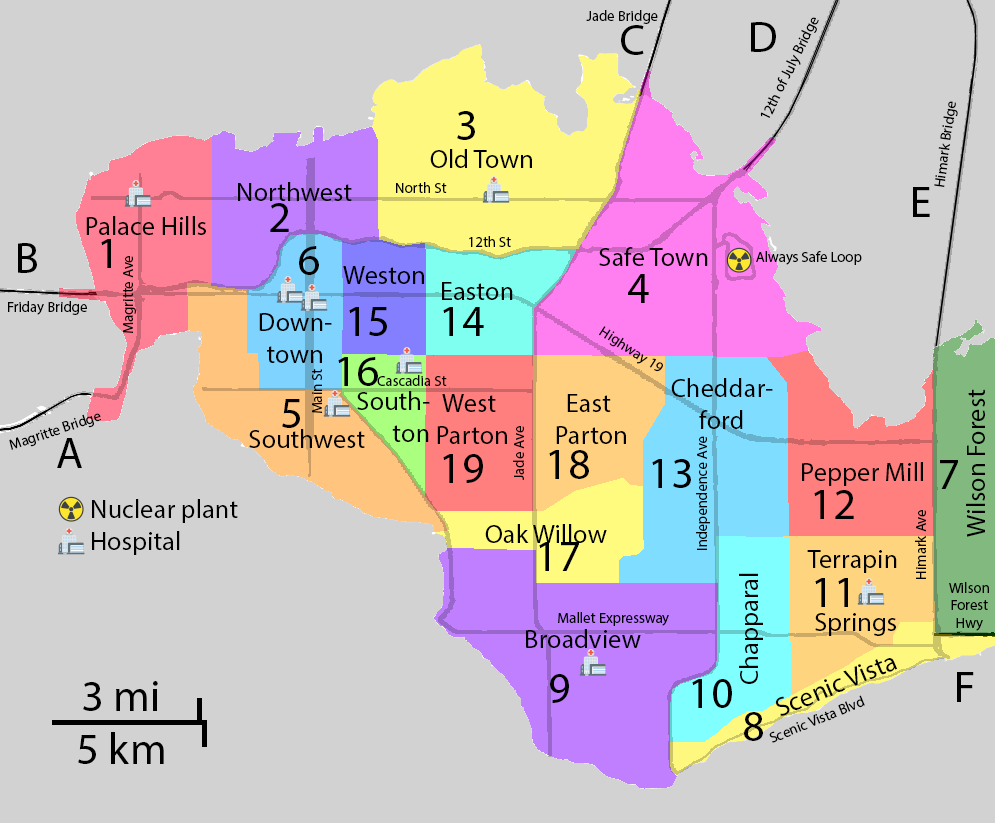
\includegraphics[width=\textwidth]{Images/map.png}
		\caption{St.Himark Neighborhood Map}
		\label{fig:map}
	\end{minipage}%
	\begin{minipage}{0.5\textwidth}
		\centering
		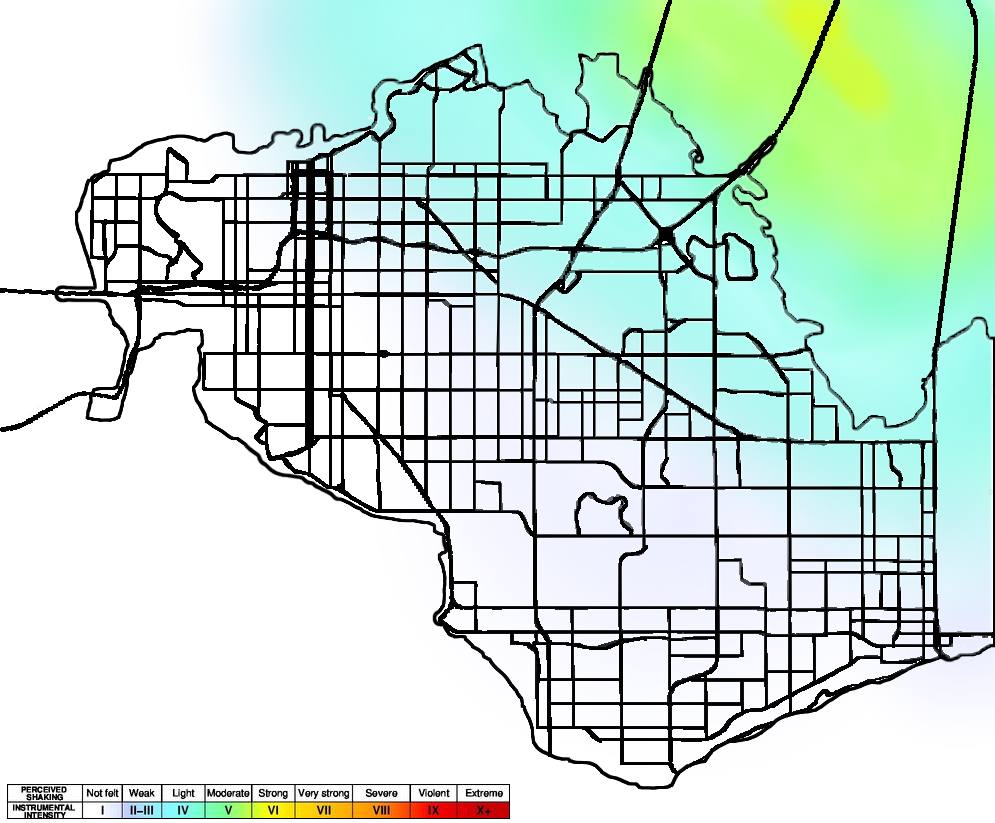
\includegraphics[width=\textwidth]{Images/shakemap.png}
		\caption{St.Himark Shake Map}
		\label{fig:shakemap}
	\end{minipage}
\end{figure} 

Based on preliminary visual comparison, it can be noted that the cities Old Town (location Id: 3), Safe Town (location Id: 4), Wilson Forest (location Id: 7) and Pepper Mill (location Id: 12) are the ones that are experiencing the maximum shake among all the cities. On the given scale, they are experiencing Moderate(\Romannum{4}) shake. 
	
\subsection{Prioritizing Neighborhood Response:}
During a Calamity, the foremost concern is to keep the casualties to a minimum. This means deploying immediate medical assistance to disaster struck areas. There are a total of 7 hospitals spread across St. Himark as shown in Figure \ref{fig:map}.  \\

Figure \ref{fig:medical} shows the damage hospitals sustained in different localities. As expected, the hospital at Old Town (location Id: 3) is the one with maximum reported damage. The emergency responders probably have to divert all possible injured to Downtown (location Id: 6) which has sustained about half the medical building damage as compared to Old Town.  \\

Transporting injured to different locations comes at the cost of Time. It is only possible to transport the minorly injured to farther locations. This transportation can work only if the roads and bridges are intact. Let us take a look at the damages the roads have taken at different location.  \\

Figure \ref{fig:road} represents the average reported damage roads and bridges sustained during the earthquake. It is to be noted that the graph peaks at Location 8, Scenic Vista, which was safe from the earthquake according to the shake map. However, Old town has sustained an average reported damage of 7.26 out of 10, which is quiet a lot. This could cause major delays in transporting people out of Old Town. Relocating only the non-fatal injuries might be a good idea. Safe Town (location 4) is another major concern. It does not have its own hospital and the average road damage is reported at 4.21. This is not the worst, but certain roads might be inaccessible. Proper communication between the emergency response team can reduce the transportation time. The nearest hospitals to Safe Town are located at Terrapin Springs (location 11), Broadview (location 9) and Southton (location 16). \\ 


%Medical Damage Image
\begin{figure}[H]
\centering
	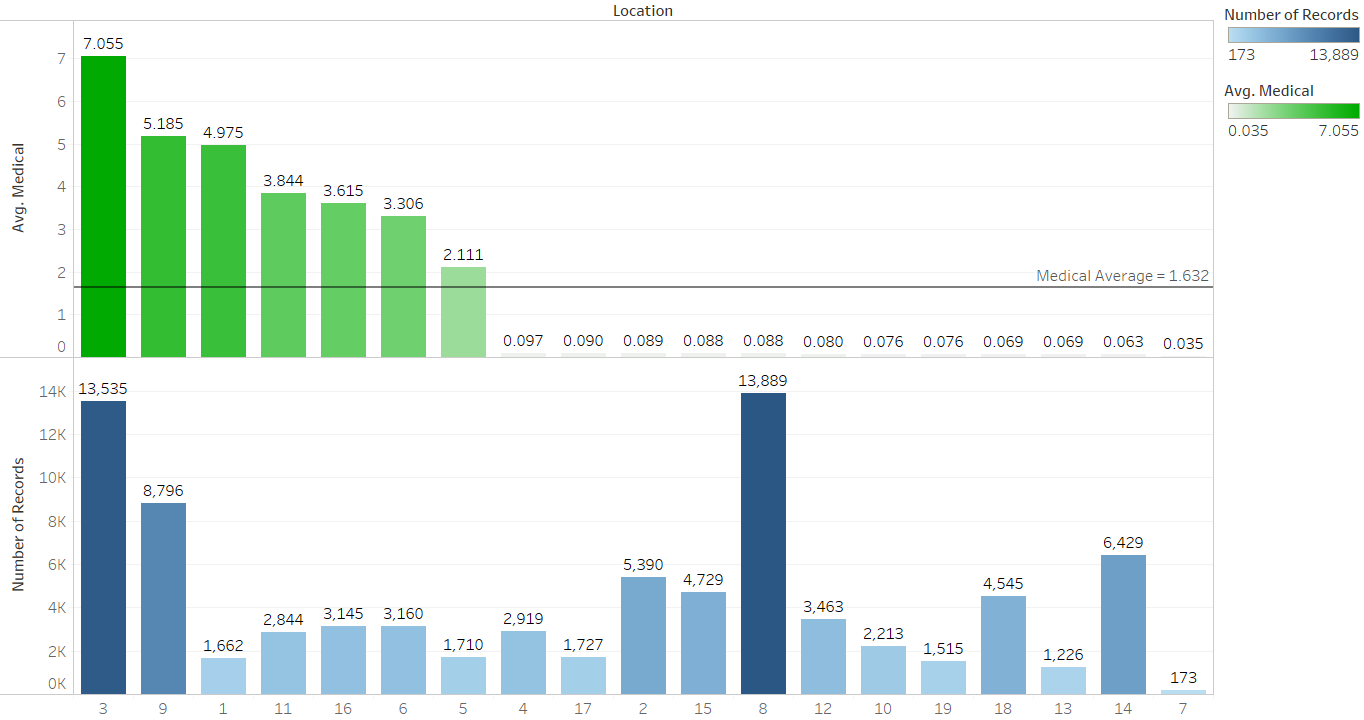
\includegraphics[width=\linewidth]{Images/medical.png}
	\caption{Location Vs Reported Medical Building Damage }
	\label{fig:medical}
\end{figure}

%Road Damage image
\begin{figure}[H]
\centering
	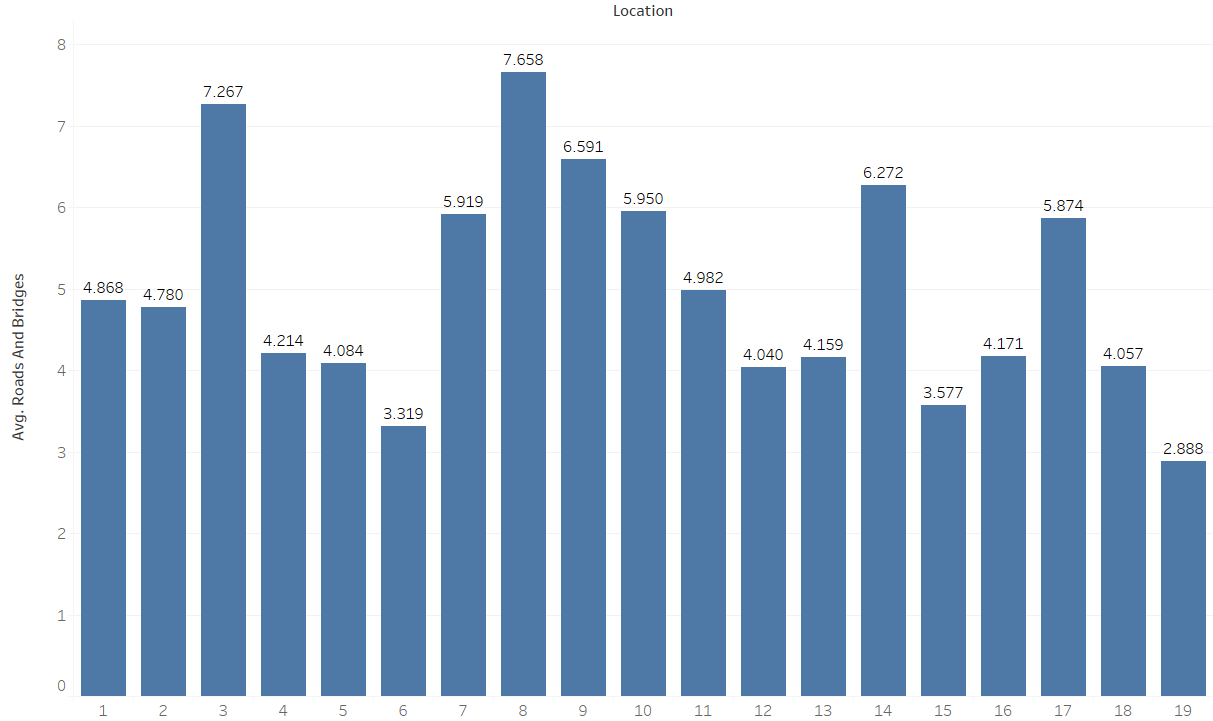
\includegraphics[width=\linewidth]{Images/Road.png}
	\caption{Location Vs Reported Roads and Bridges Damage }
	\label{fig:road}
\end{figure}
 
 %Medical and Road images combined
 \begin{figure}[H]
\centering
	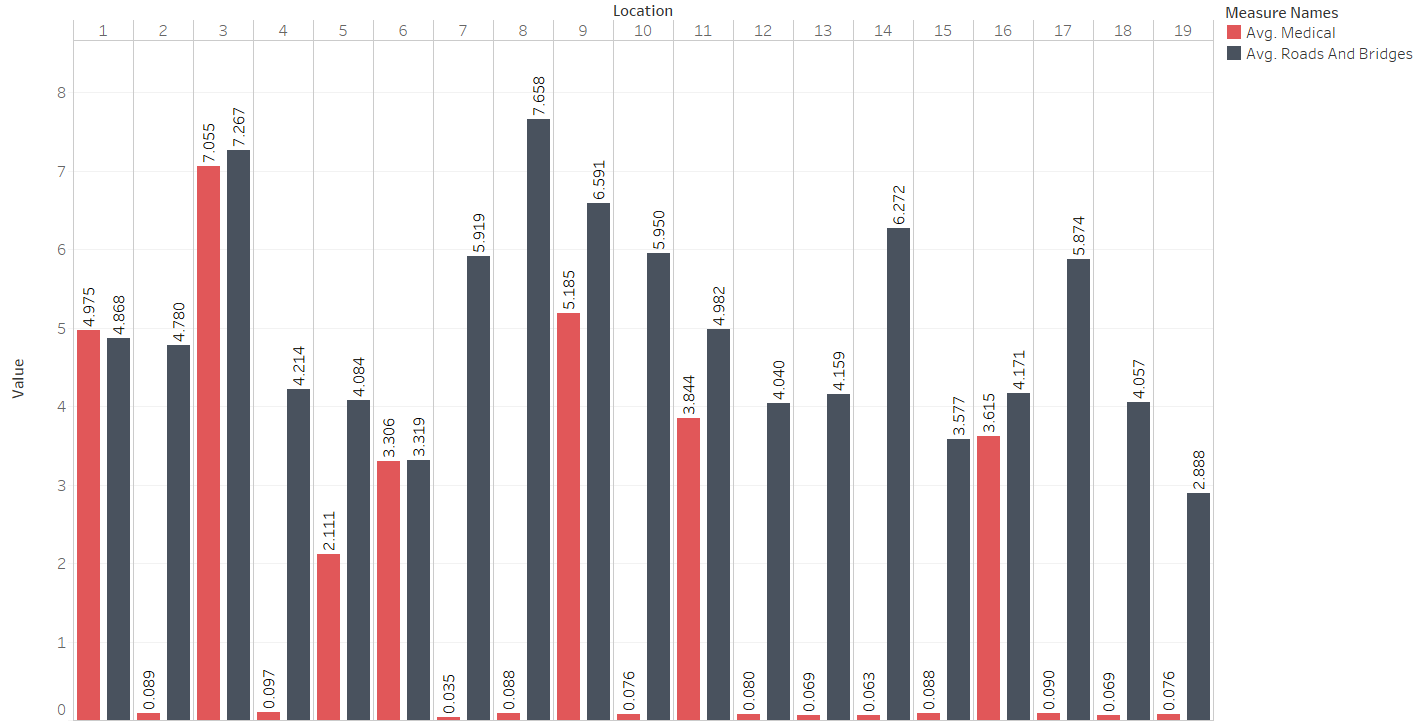
\includegraphics[width=\linewidth]{Images/MedRoad.png}
	\caption{Reported damages to Roads and Medical facilities at different locations of St. Himark }
	\label{fig:medroad}
\end{figure}
 
 Figure \ref{fig:medroad} shows the reported damages of Roads and Medical Facilities next to each other. This plot is helpful in scouting out the fastest route to transport the injured from Old Town (Location Id: 3) and Safe Town (Location Id: 4), as these two have taken severe damage. 
 
 \subsection{Damages to the community:}
 \label{subsec:damage}
 Even though the North-Eastern side of the community was hit directly by the earthquake, the entire community is facing the consequences. Even the Cities farthest from the earthquake\rq{}s epicenter took considerable amount of damage. 
 
 %All damage Aggregate Image
\begin{figure}[H]
\centering
	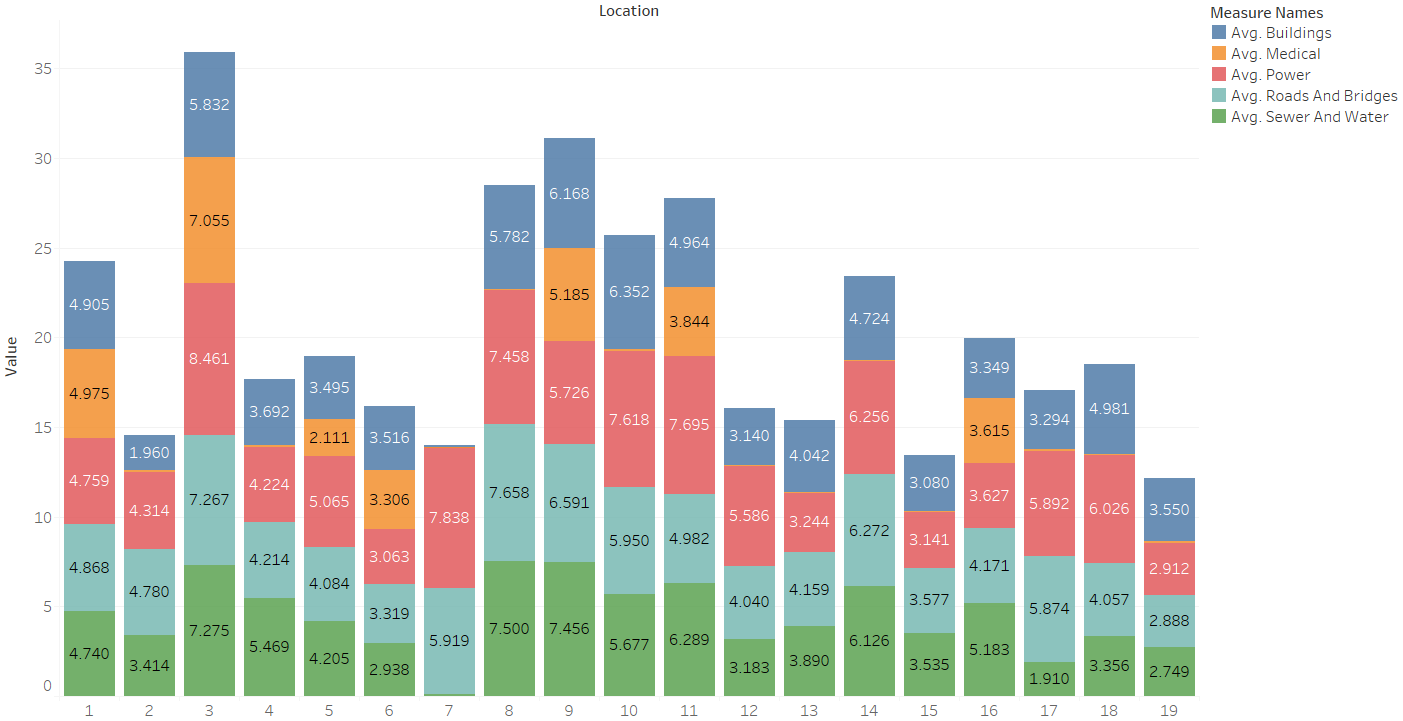
\includegraphics[height=0.43\linewidth, width=\linewidth]{Images/AllDamage.png}
	\caption{Collective damage to different locations in the Community}
	\label{fig:alldamage}
\end{figure}
 
 Figure \ref{fig:alldamage} shows the collective damage reported from different locations in the community. Again, to no surprise, Old Town (location 3) has taken the overall highest damage. Broadview (location 9) takes the second place, even though it resides quiet further away in the earthquake\rq{}s shake map (Figure \ref{fig:shakemap}). 

%Shake intensity Image
\begin{figure}[H]
\centering
	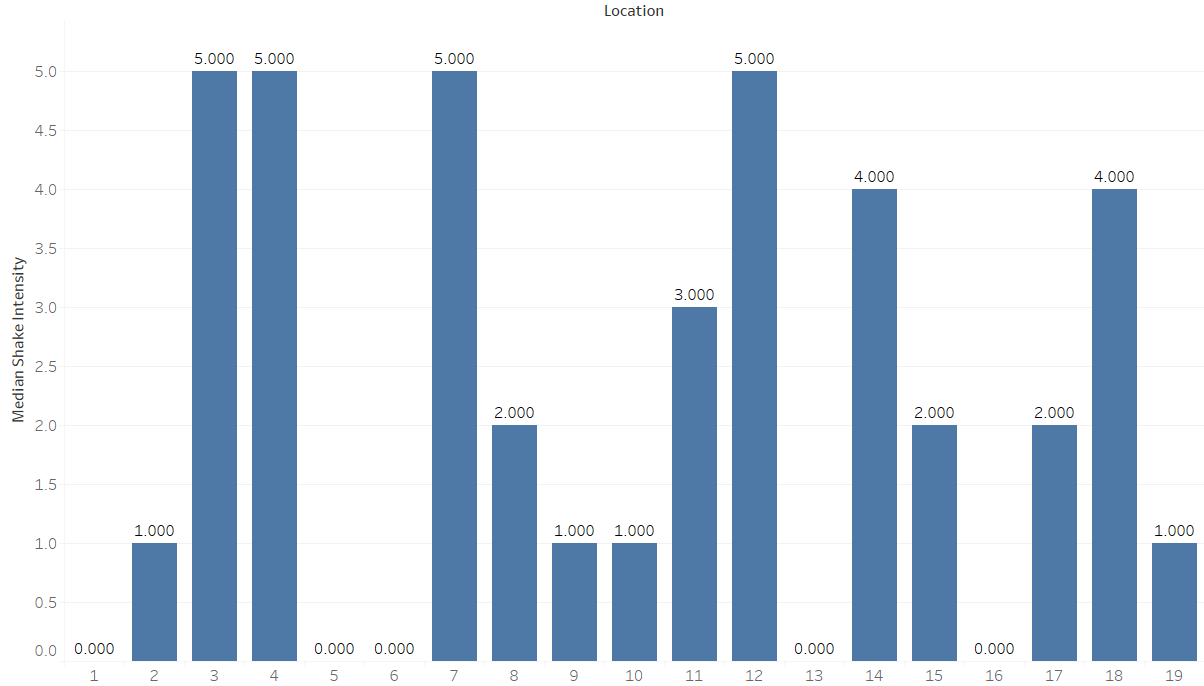
\includegraphics[height=75mm, width = 0.8\linewidth]{Images/ShakeInt.png}
	\caption{Median of Shake Intensity at different Locations}
	\label{fig:shakeint}
\end{figure}

Figure \ref{fig:shakeint} shows the median of the shake intensities experienced at different locations. This graph gives us an idea of how much each cities experienced the earthquake compared to its neighbors. Locations 3, 4, 7 and 12 took a direct hit, thus they peak the graph. Locations 14 and 18 takes the second place as expected. 

%All damage Image
\begin{figure}[H]
\centering
	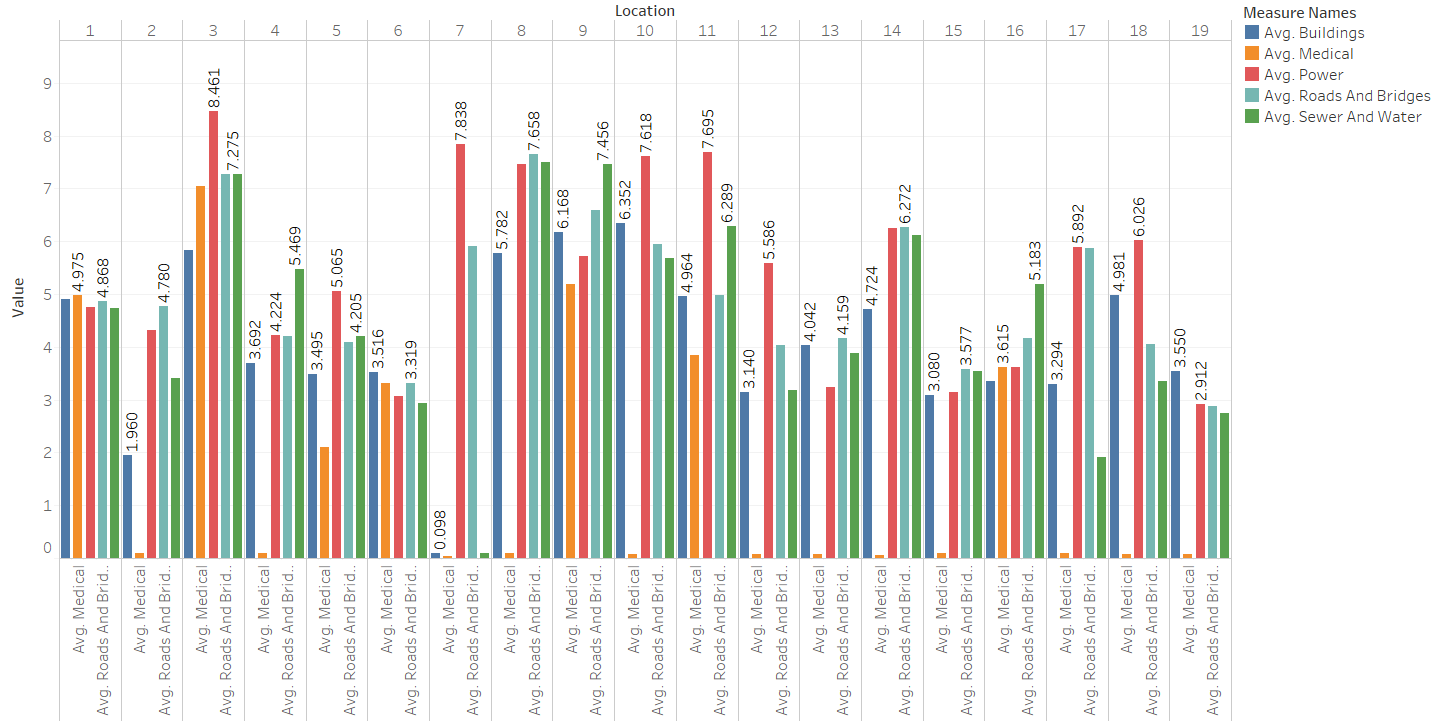
\includegraphics[width=\linewidth]{Images/AllSeperate.png}
	\caption{Damages to different aspects of the city}
	\label{fig:allseperate}
\end{figure}

Figure \ref{fig:allseperate} helps us to compare the damages to different aspects of the city with its neighbors.  It appears that power systems have taken the maximum damage in majority of the cities. It can also be noted that Location 7, Wilson Forest has minimum damage to everything except roads and power. This could mean that the location has less human population thus the need for hospitals and other buildings are scarce. \\

This is an important observation because, till now, all the analysis was done based on the assumption that the population on all the cities were almost the same. But this may not be the case. Also, the number of reports from different cities registered were not taken into consideration. This may cause inaccuracies in the conclusions drawn form the raw damage reports taken from the RUMBLE application. 

 \newpage
\begin{centering}
	\section{Conclusion}
\end{centering}

Based on the visualizations of the damages caused to the medical facilities and roads, it seems appropriate to deploy medical help to Safe Town and Old Town as soon as possible. Safe Town being deprived of its own hospital, needs the injured to be transported to the closest medical facility whereas Old Town may have problems dealing with the injured as the hospitals may have taken severe damage due to the earthquake. \\

These conclusions are drawn on the assumption that all cities have equal reports registered. But as seen in section \ref{subsec:damage}, there might be an imbalance in the reports registered. 

\begin{figure}[H]
\centering
	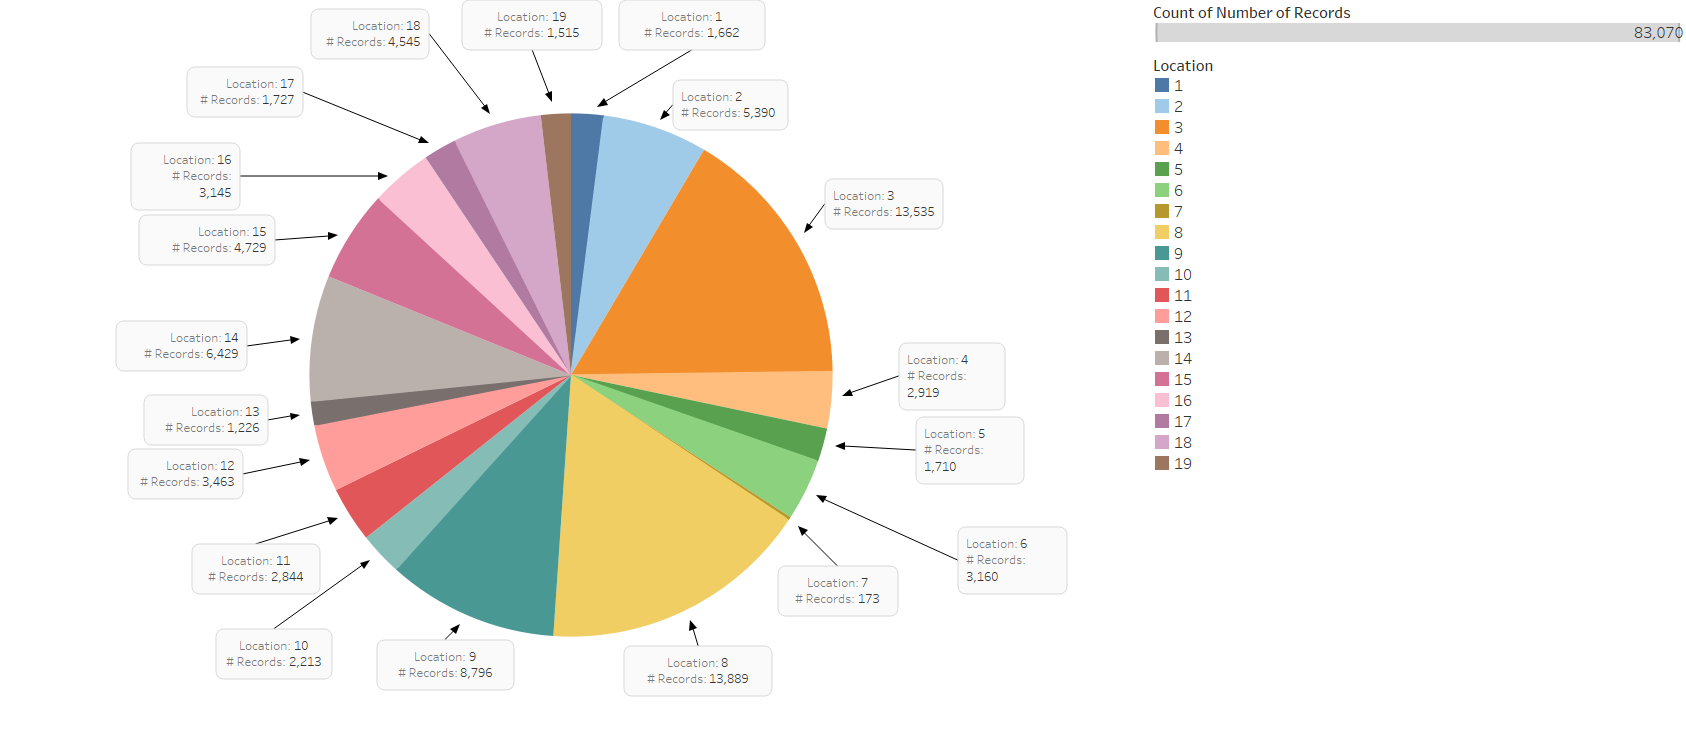
\includegraphics[width=\linewidth]{Images/RecordPercentile.png}
	\caption{Compression of number of damage reports registered from different locations}
	\label{fig:regrecords}
\end{figure}

Figure \ref{fig:regrecords} shows the number of reports registered from different locations. Out of the total 83,070 registered damage reports, 13,889 comes from location 8 and 13,535 comes from location 3. This contributes to around 16.72\% and 16.29\% of the total reports. Compared to these, location 7 with only 173 reports, contributes only a mere 0.21\%. \\

This irregularity in the reports could be the reason for the unexpected results in Figure \ref{fig:road}. This result brings an important question to light. \\

\noindent
\textbf{How reliable are the damages reports recorded by the citizens of St.Himark? } \\

\noindent
This problem will be addressed in the Part 2 of the MiniChallenge 1. 





\end{document}


